\chapter{Nuevos operadores para STL}
\label{cha:stl}

\section{Signal Temporal Logic}
% Definición, sintaxis y semántica de los operadores.
\textit{Signal Temporal Logic} (STL) \cite{STL} es un tipo de lógica temporal especializada en el análisis de señales reales analógicas. STL permite expresar características sobre la evolución de algún atributo físico, como la velocidad o temperatura. Por tanto, como punto de partida, STL requiere una muestra o traza de ejecución sobre la que comprobar las hipótesis.

La lógica distingue dos tipos de situaciones: propiedades que se satisfacen en un \textit{estado} o momento puntual de la traza de ejecución, o propiedades de \textit{camino} que se evalúan a lo largo de una secuencia de eventos. STL proporciona operadores para recorrer los diferentes estados del sistema y comprobar en qué momentos se cumplen las propiedades.

Por ejemplo, la proposición atómica $v > 120$ mostraría los instantes en los que la velocidad supera los $120$. Los operadores de camino enriquecerían esa expresión para analizar si la velocidad se sobrepasa puntualmente en algún momento (\textbf{F})uturo del viaje, (\textbf{G})eneralmente a lo largo de todo el recorrido, o permanece constante hasta (\textbf{U}ntil) que se incrementa a un nuevo valor. 

Formalmente, la gramática básica de STL comprende los siguientes operadores:

$$ \varphi \ := \ \mu \ |\ \neg \varphi \ |\ \varphi_{1} \lor \varphi_{2} \ |\ \varphi_{1} U_{[t_1, t_2]} \varphi_{2}$$

Donde $\mu$ representa las proposiciones atómicas, en forma de desigualdades sobre la señal muestreada (p.ej., $\mu := v > 120$); y $\varphi$ las especificaciones sobre los caminos. El resto de los operadores se componen a partir de los operadores precedentes, donde $t_1, t_2 \in \mathbb{R}_{\geq 0}$ son marcas temporales que definen el intervalo de monitorización respecto al instante inicial, siendo $t_1 \geq t_2$. 

% Operador futuro y general

% $$ F_{[a,b]} \varphi \equiv \top U_{[a,b]} \varphi $$
% $$ G_{[a,b]} \varphi \equiv \neg F_{[a,b]} \neg \varphi $$

\begin{align*}
F_{[a,b]} \varphi \equiv \top U_{[a,b]} \varphi & &
G_{[a,b]} \varphi \equiv \neg F_{[a,b]} \neg \varphi
\end{align*}

Existen versiones extendidas que permiten analizar aspectos cuantitativas con STL, por ejemplo, los valores máximos/mínimos \cite{TACAS_19} o integrales en un intervalo, o calcular la derivada en un punto \cite{Stl_Der_Int}.


Las especificaciones en STL se \textit{compilan} en un monitor que supervisa la ejecución del sistema (p. ej., el sensor de velocidad de un vehículo). Algunos intérpretes de STL son AMT \cite{AMT2} (sintaxis básica) y STLEval \cite{StlEval} (sintáxis básica y operadores de min/max). En este proyecto, implementaremos en STLEval los operadores cuantitativos de STL que permiten calcular integrales y derivadas sobre una señal, según la definición propuesta en \cite{Stl_Der_Int}.

\section{STLEval}
%Lenguaje utilizado en STLEval (C++), etc.
STLEval es una herramienta capaz de manejar tanto expresiones STL básicas, que devuelven señales Booleanas, como ciertas extensiones cuantitativas, que transforman la señal de entrada en una nueva señal continua (operadores de min/max). Por estos motivos, así como su eficiencia (está escrita en en C++) STLEval se ha tomado como punto de partida para implementar los operadores cuantitativos de STL que permiten calcular integrales y derivadas sobre una señal, según la definición propuesta en \cite{Stl_Der_Int}.

% Muestreo de la señal. Representación interna en STLEval.
Internamente, STLEval representa una señal como una serie temporal, es decir, una sucesión de pares \textit{(clave, valor)} donde la \textit{clave} es una marca temporal y el \textit{valor} representa la magnitud física en ese momento. La imagen \ref{fig:senal} ilustra la señal original y su representación interna en STLEval. 

\begin{figure}
\centering
  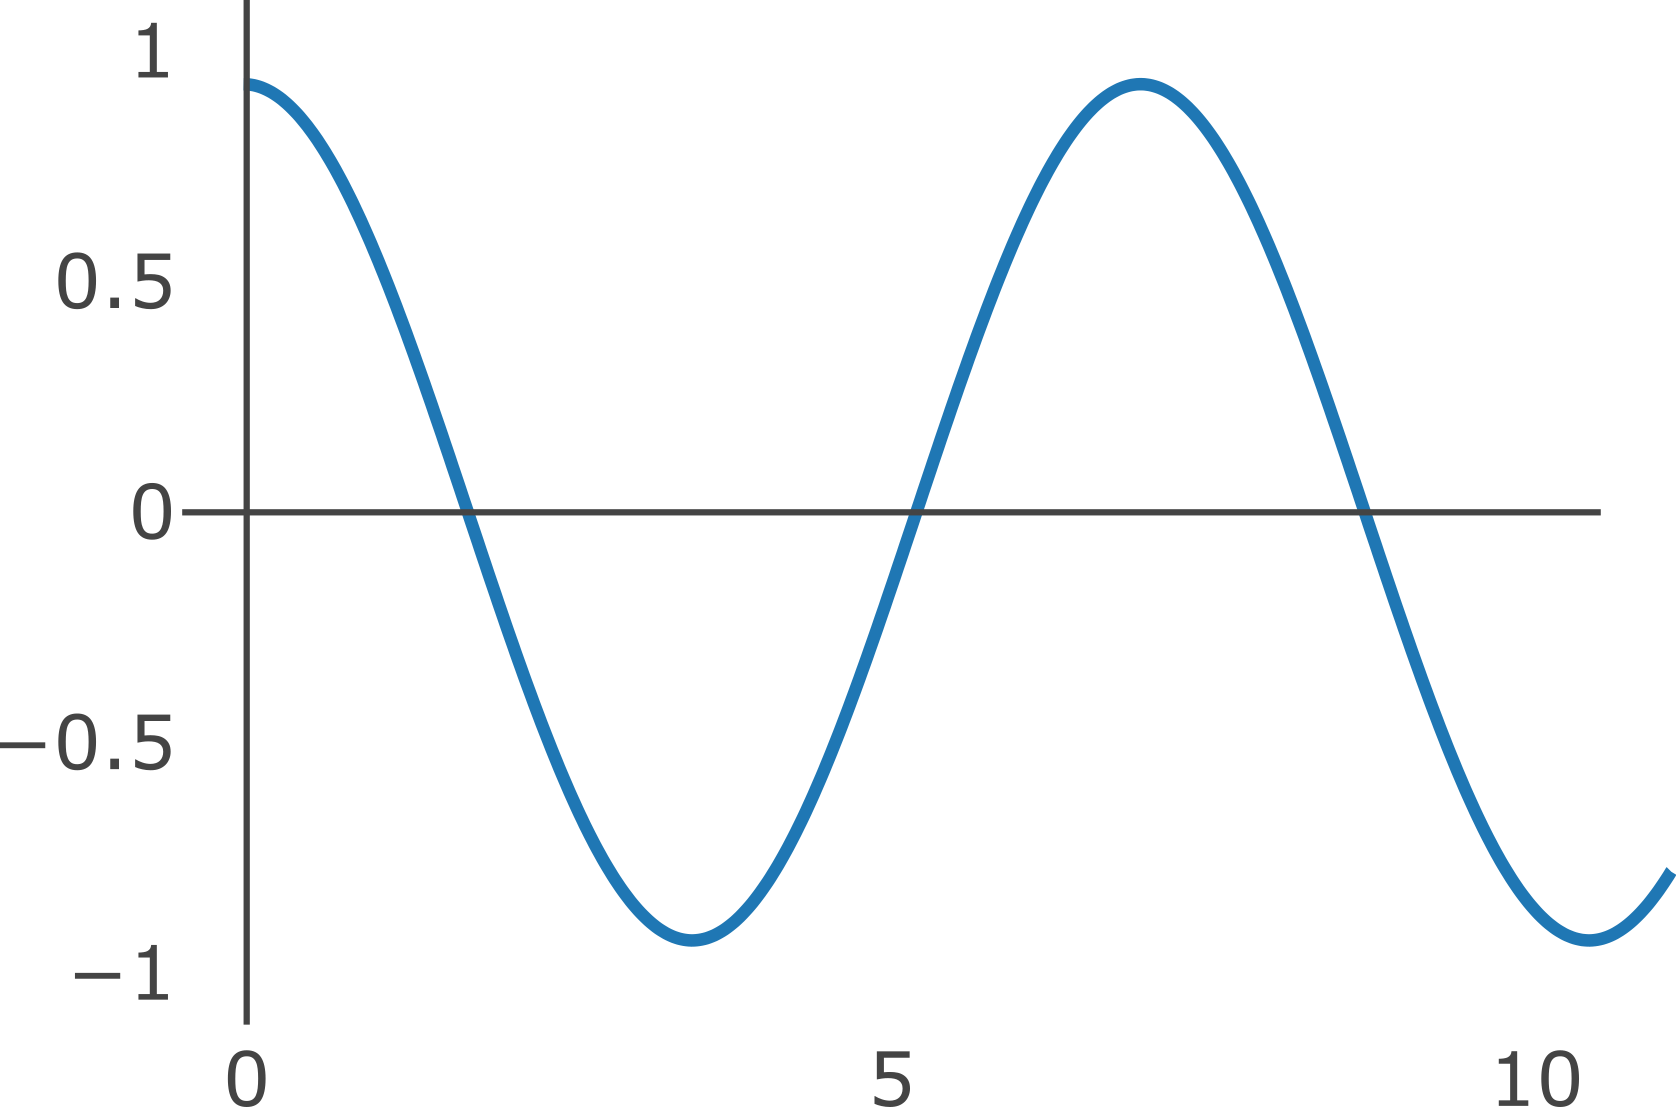
\includegraphics[width=.4\linewidth]{images/senal_original} \hfill
  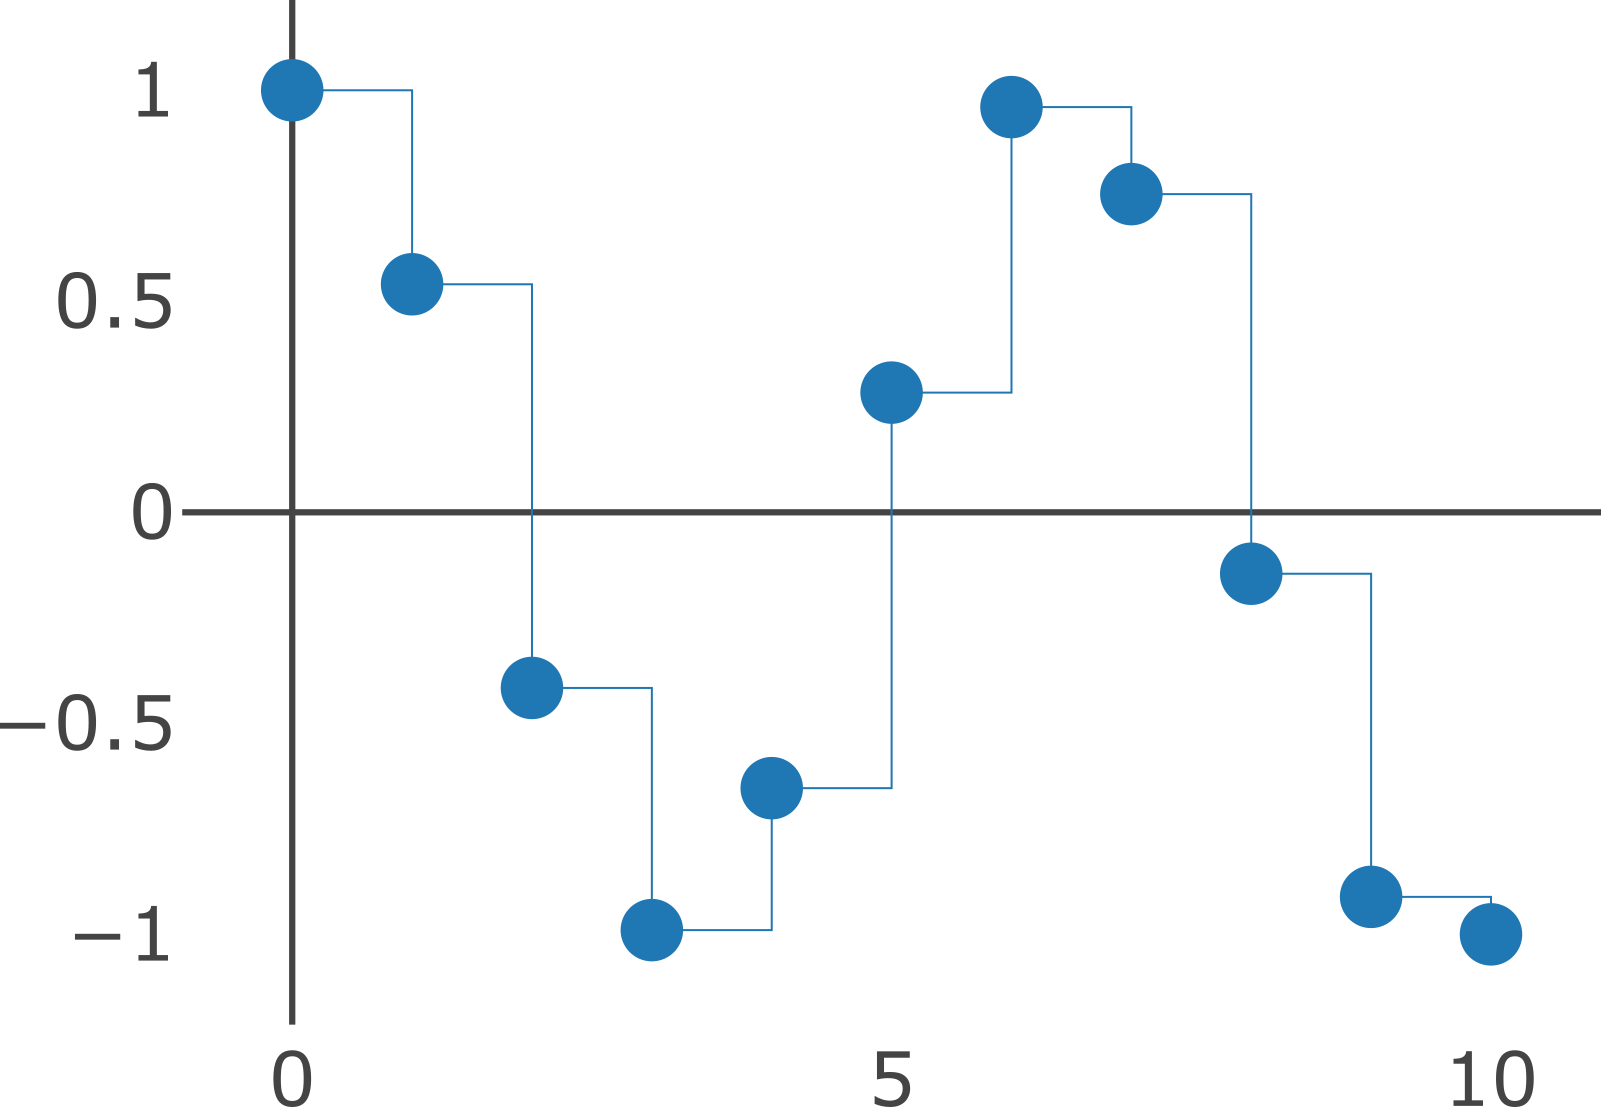
\includegraphics[width=.4\linewidth]{images/senal_muestreada}
\caption{Señal original y su reconstrucción.}
\label{fig:senal}
\end{figure}

\section{Definición de los nuevos operadores}

El cálculo de la derivada e integral se aproximan mediante las siguientes expresiones matemáticas, donde $\mathbf{x}$ representa la señal completa, $\mathbf{x}_{\tau}$ es el valor de la señal en el instante $\tau$, y $\mu^d_{+}$ ($\mu^d_{-}$) representan la aproximación de la derivada por la derecha (izquierda) del instante temporal en cuestión:

\begin{align*}
\mu^d_{+} &= \frac{dg(\mathbf{x})}{dt^+} \geq c & & \mu^i_{[a,b]} = \int^{b}_{a} g(\mathbf{x}_{\tau}) \delta \tau \geq c \\
\mu^d_{-} &= \frac{dg(\mathbf{x})}{dt^-} \geq c &
\end{align*}

Dado que internamente STLEval representa las señales reales como una serie numérica de tiempo discreto, aproximamos como:

\begin{align*}
\mu^d_{+} &= g(\mathbf{x}_{(k + 1) \delta t}) - g(\mathbf{x}_{k \delta t}) \geq c \delta t & & \mu^i_{[a,b]} = \sum^{k + b / \delta t - 1}_{k' = k + a / \delta t} g(\mathbf{x}_{k' \delta t}) \delta t \geq c \\
\mu^d_{-} &= g(\mathbf{x}_{k \delta t}) - g(\mathbf{x}_{(k - 1) \delta t}) \geq c \delta t & 
\end{align*}

Gráficamente, la derivada se interpreta como la pendiente entre dos puntos consecutivos de la señal; y la integral como el sumatorio del área de los rectángulos con base  $\delta t$ contenidos en el intervalo (Figura \ref{fig:der_int}). 

\begin{figure}
\centering
  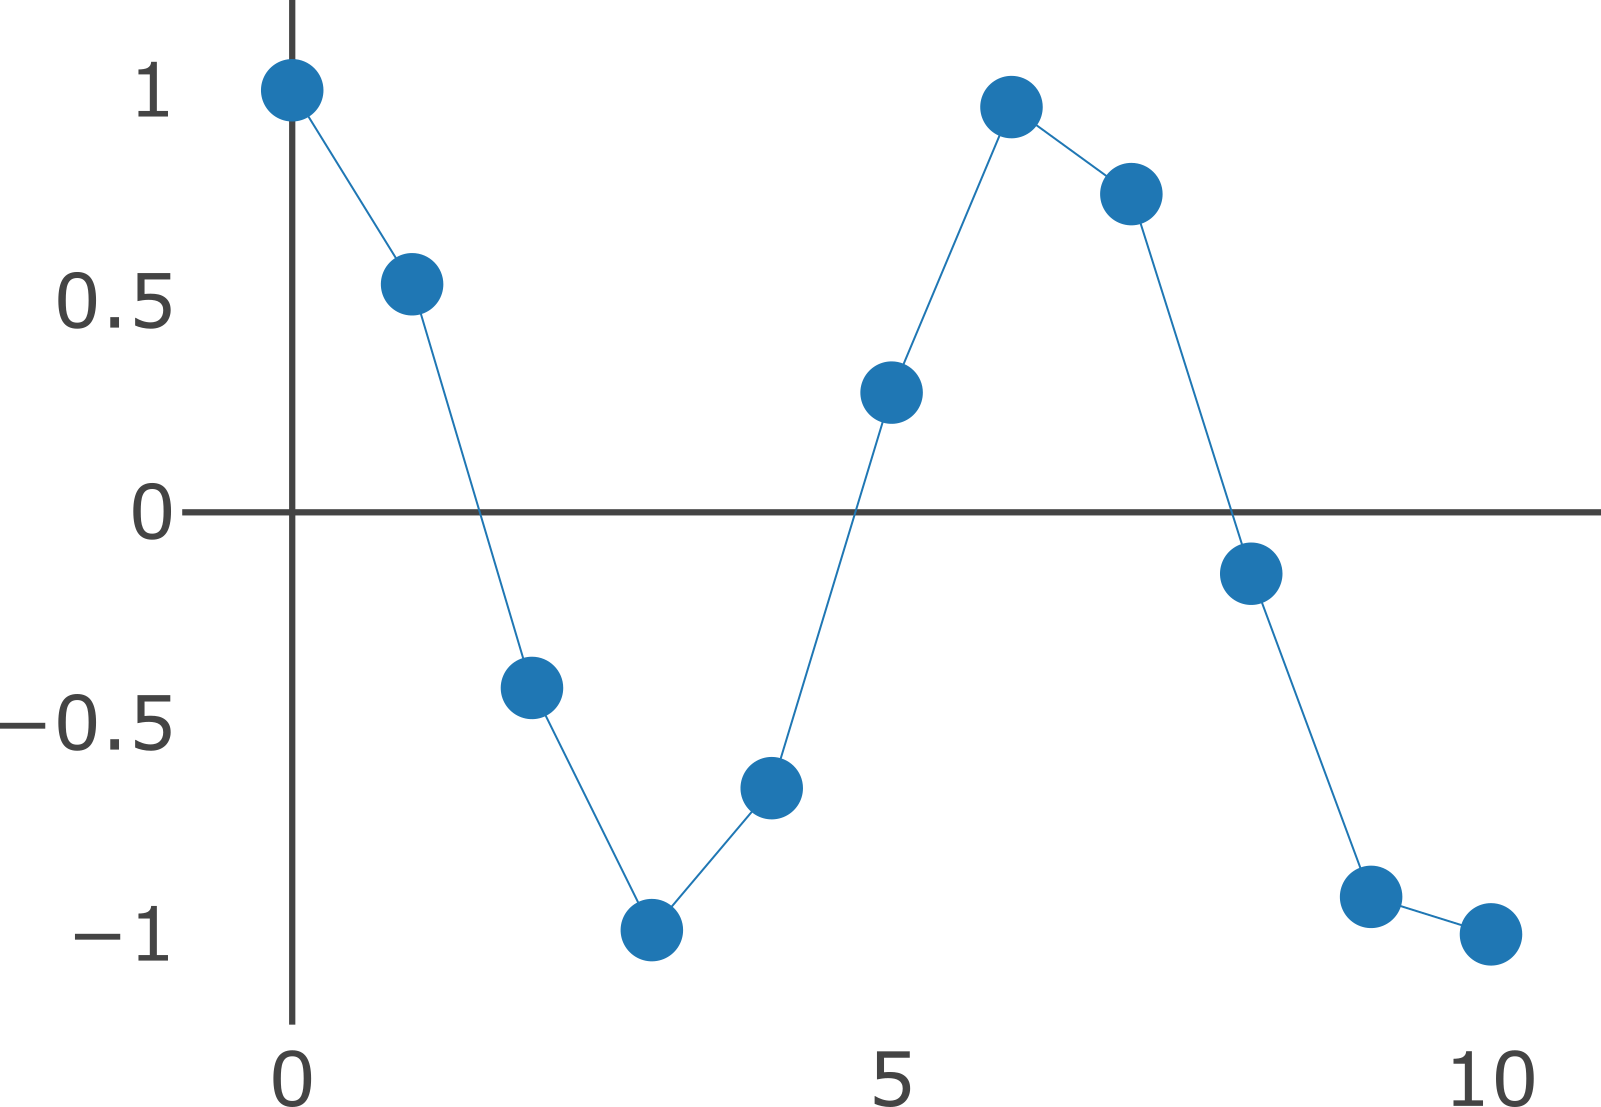
\includegraphics[width=.4\linewidth]{images/derivada} \hfill
  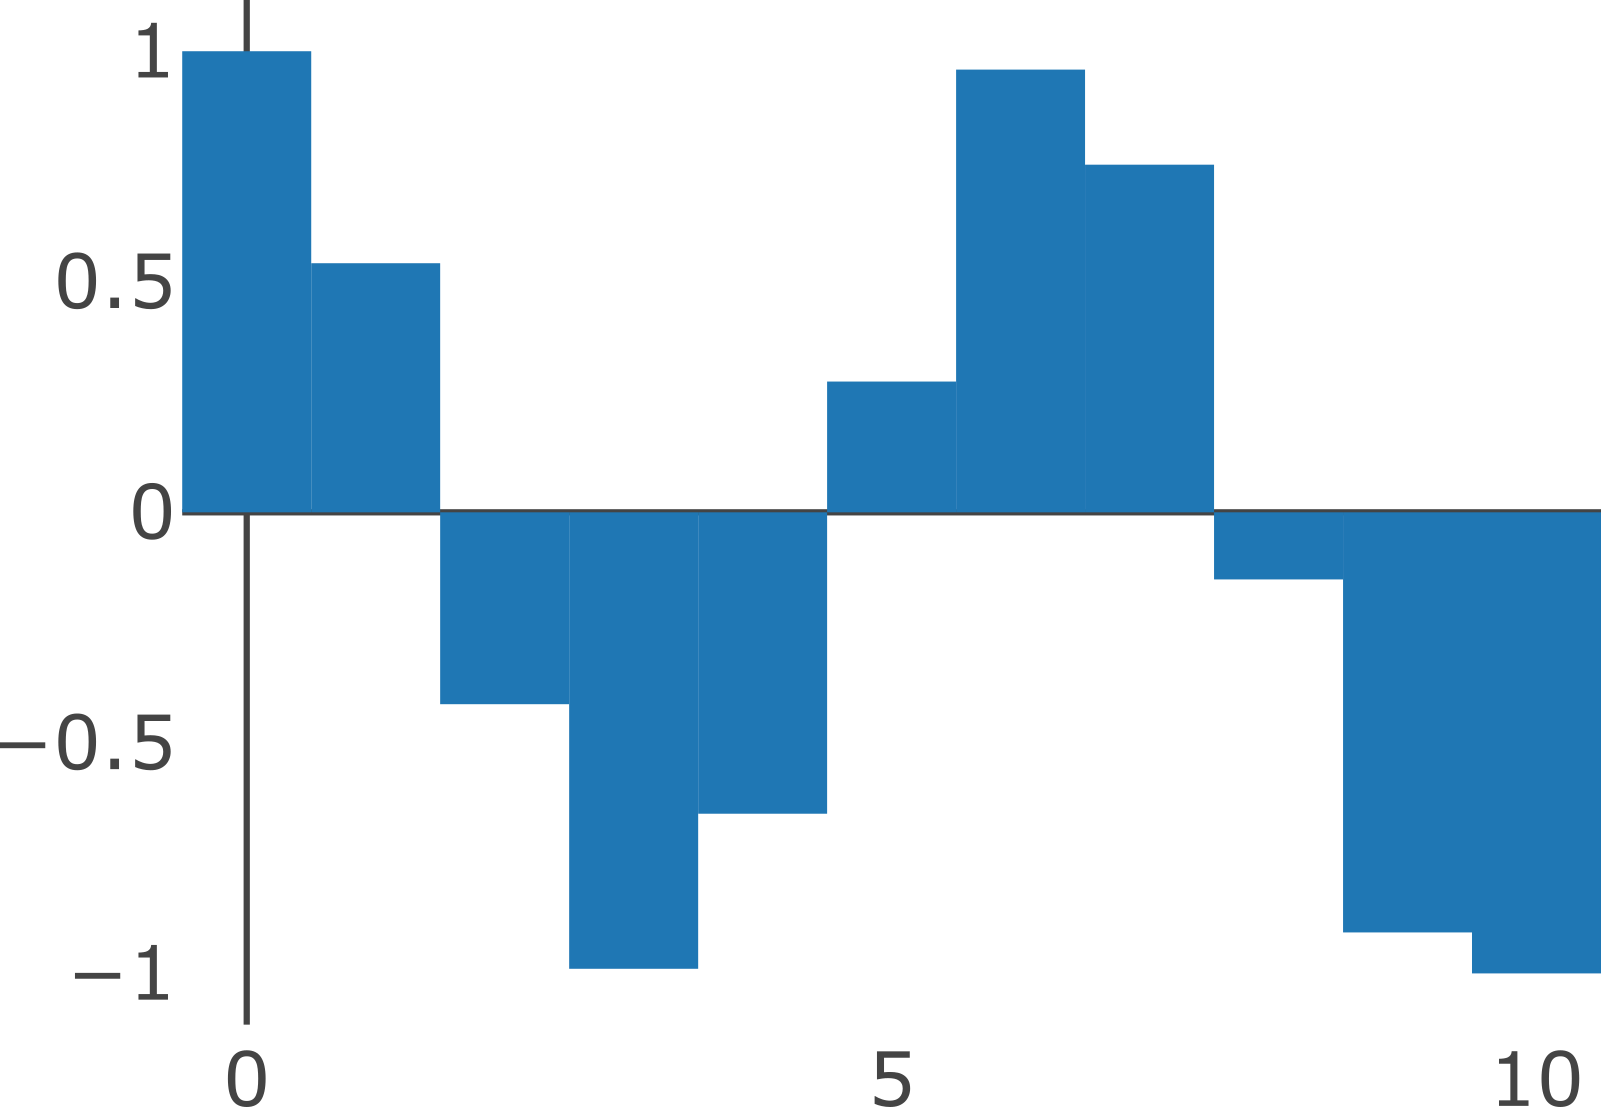
\includegraphics[width=.4\linewidth]{images/integral}
\caption{Interpretación de la derivada e integral.}
\label{fig:der_int}
\end{figure}

\section{Integración con ParetoLib}
ParetoLib \cite{FORMATS_19, ParetoLib} es una librería de minería que recibe una especificación paramétrica o plantilla en STL y devuelve el rango de valores de las variables para las que la propiedad se satisface o invalida. 

Internamente, ParetoLib implementa un algoritmo de búsqueda que guía el aprendizaje y evalúa instancias concretas de la fórmula temporal a través de la herramienta STLEval.

ParetoLib está escrito en Python. El código fuente \ref{list:paretolib_example} ilustra la forma de invocar a la librería.

Dada una señal triangular \ref{} y la especificación STL X, la imagen \ref{•} muestra en las configuraciones de los parámetros X que satisfacen la propiedad (región en verde) y las que lo falsifican (región en rojo).

% Contribuciones
En este proyecto, hemos actualizado los binarios y librerías dinámicas de STLEval que incorpora ParetoLib para dar soporte a las nuevas operaciones de derivación e integración. Además, hemos implementado una interfaz gráfica que abstrae la complejidad de invocar al código fuente \ref{list:paretolib_example} y resume la mayor parte de las opciones de configuración del algoritmo de minería.

\jicomment{TODO:
\begin{itemize}
\item Referenciar a la rama de ParetoLib/GUI donde se engloban los cambios de la GUI + los nuevos binarios de STLEval
\item Describir un ejemplo de STL con parametros sobre un operador derivada/integral. Por ejemplo `` I [0, 20] sin(x) `` sería 0; ``F D sin(x) > 0`` sería True, ...
\end{itemize}
}

\lstinputlisting[language=python,
		style=mystyle,
		label={list:paretolib_example},
		caption={}]
		{code/python/example2d_derivative.py}